\chapter{Проектирование и создание
представлений, встроенных функций
и синонимов}
\section{Проектирование и реализация
представлений и встроенных функций }

В SQL представления используются для хранения и повторного использования запросов к базе данных. Представления могут использоваться практически для тех же целей, что и таблицы.



\begin{lstlisting}[label=lst:funcReturn, language=sql]
	CREATE VIEW Sales.OrderTotalsByYear
		WITH SCHEMABINDING
	AS 
		SELECT
			YEAR(O.orderdate) AS orderyear,
			SUM(OD.qty) AS qty
		FROM Sales.Orders AS O
		JOIN Sales.OrderDetails AS OD
		ON OD.orderid = O.orderid
		GROUP BY YEAR(orderdate); 
\end{lstlisting}

Это представление создано с использованием параметра представления
SCHEMABINDING, который гарантирует, что структуры базовых таблиц не могут
быть изменены без удаления представления. 

\begin{figure}[h!]
	\begin{center}
		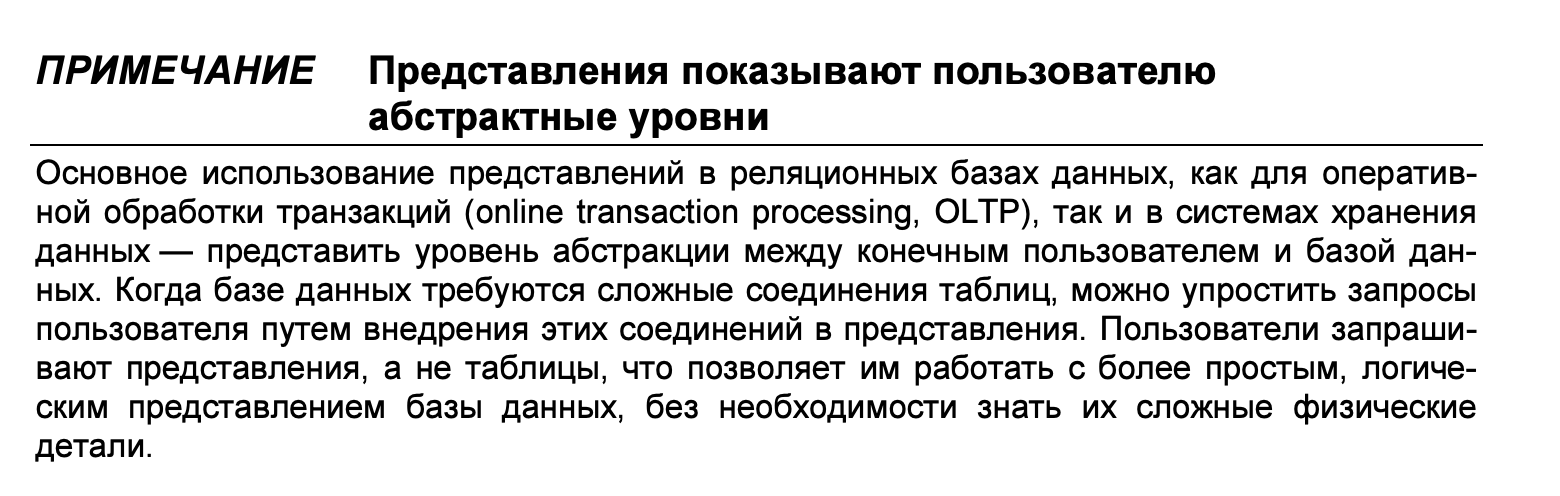
\includegraphics[width=0.9\textwidth]{img/advice16.png}
	\end{center}
	\captionsetup{justification=centering}
\end{figure}


\begin{figure}[h!]
	\begin{center}
		
\includegraphics[width=0.9\textwidth]{img/advice17.png}
	\end{center}
	\captionsetup{justification=centering}
\end{figure}

\subsection{Параметры представления}

Можно добавить следующие параметры представления в любой комбинации. 
\begin{itemize}
	\item  С помощью предложения WITH ENCRYPTION можно указать, что текст представления должен быть сохранен в неявном виде (это не строгое шифрование). Это затрудняет для пользователей раскрытие текста инструкции SELECT представления. 
	\item  Предложение WITH SCHEMABINDING, как уже говорилось ранее, привязывает представление к схемам базовых таблиц: нельзя изменить определения схем таблицы без удаления представления. Это защищает представление от повреждения в результате изменения структур таблиц. 
	\item Предложение WITH VIEW\_METADATA, когда оно указано, возвращает метаданные
	представления, а не базовой таблицы.
\end{itemize}


\subsection{Предложение WITH CHECK OPTION}

Предложение WITH CHECK OPTION ограничивает модификации только строками, которые удовлетворяют критериям фильтра. 

\subsection{Ограничения в представлениях}
Представления имеют некоторые ограничения, перечисленные далее. 

\begin{itemize}
	\item В представлении нельзя добавить предложение ORDER BY в инструкции SELECT.
	Представление должно выглядеть точно так же, как таблица, а таблицы в реляционных базах данных содержат наборы строк. Сами по себе наборы не упорядочены, хотя можно применить к ним сортировку в результирующем наборе
	с помощью предложения ORDER BY. Аналогично, строки таблиц и представлений
	в SQL Server не имеют логического порядка, хотя их можно упорядочить, добавив предложение ORDER BY в самой внешней инструкции SELECT при доступе
	к представлению.
	\item Представлению нельзя передавать параметры. Аналогично, представление не
	может ссылаться на переменную внутри инструкции SELECT. 
	\item Представление не может создать таблицу, как постоянную, так и временную.
	Иными словами, в представлении нельзя использовать синтаксис SELECT/INTO. 
	\item Представление может ссылаться только на постоянные таблицы; оно не может
	ссылаться на временную таблицу. 
\end{itemize}

\begin{figure}[h!]
	\begin{center}
		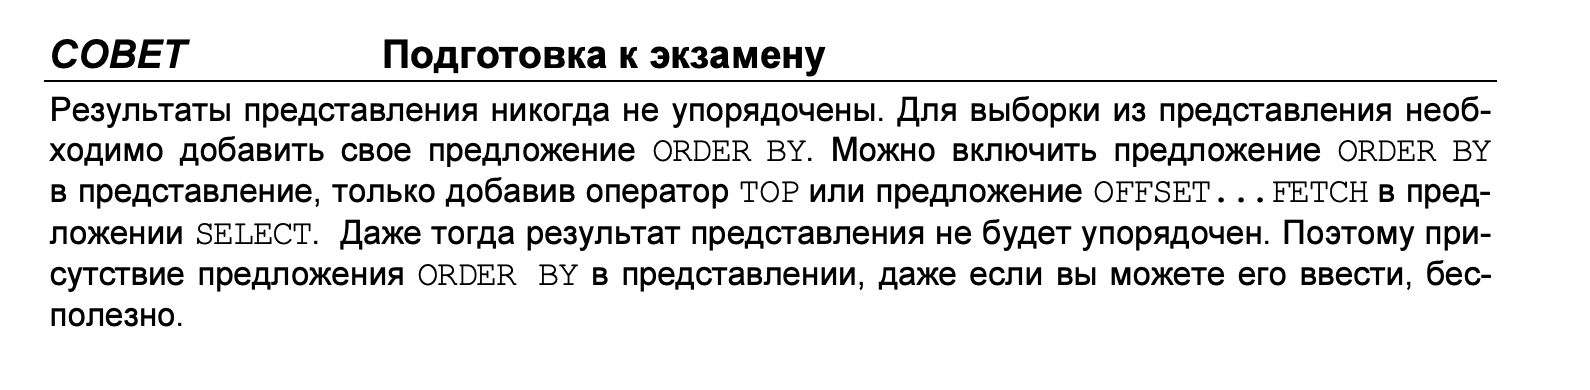
\includegraphics[width=0.9\textwidth]{img/advice18.png}
	\end{center}
	\captionsetup{justification=centering}
\end{figure}

\subsection{Индексированные представления}

Можно создать уникальный кластеризованный индекс на представлении и таким
образом материализовать данные. В этом случае хранится не только определение
представления. На диске сохраняются фактические результаты запроса, в структуре
кластеризованного индекса. 


\subsection{Выполнение запросов из представлений}

При выполнении запроса из стандартного нематериализованного представления
оптимизатор запросов SQL Server объединяет ваш внешний запрос с запросом,
встроенным в представление, и обрабатывает этот объединенный запрос. В результате, когда вы посмотрите на планы запросов для запросов, в которых выборка выполняется из представлений, то увидите в плане запроса ссылочные базовые таблицы представления; само представление не будет объектом в плане запроса. 

\subsection{Изменение представления}
Команда ALTER VIEW
просто переопределяет работу представления посредством полного повторного определения представления. 

\begin{lstlisting}[label=lst:funcReturn, language=sql]
	ALTER VIEW Sales.OrderTotalsByYear
		WITH SCHEMABINDING
   	AS
   	SELECT O.shipregion,
		YEAR(O.orderdate) AS orderyear,
		SUM(OD.qty) AS qty
   	FROM Sales.Orders AS O
	JOIN Sales.OrderDetails AS OD
	ON OD.orderid = O.orderid
   	GROUP BY YEAR(orderdate), O.shipregion; 
\end{lstlisting}


\subsection{Удаление представления}

\begin{lstlisting}[label=lst:funcReturn, language=sql]
	DROP VIEW Sales.OrderTotalsByYear;
\end{lstlisting}


\subsection{Модификация данных с помощью представления}

Ограничения:

\begin{itemize}
	\item DML-инструкции (INSERT, UPDATE и DELETE) должны ссылаться точно на одну
	таблицу за один раз, неважно, на сколько таблиц ссылается представление. 
	\item Столбцы представления должны напрямую ссылаться на столбцы таблиц и не
	являться выражениями или функциями, окружающими значение столбца. 
	\item Нельзя модифицировать столбец представления, который является вычисляемым и формируется с помощью операторов UNION/UNION ALL, CROSS JOIN, EXCEPT
	или INTERSECT. 
	\item Нельзя модифицировать столбец представления, значения которого получены
	группированием, например, с использованием предложений DISTINCT, GROUP BY и
	HAVING. 
	\item Нельзя модифицировать представление, имеющее конструкции TOP или
	OFFSET...FETCH в инструкции SELECT, вместе с предложением WITH CHECK OPTION. 
\end{itemize}

\subsection{Секционированные представления}

Если у вас нет возможности
использовать секционирование таблиц, вы можете разделить ваши таблицы вручную и создать представление, которое применяет инструкцию UNION к этим
таблицам. Результат этого называется секционированным представлением.

\begin{figure}[h!]
	\begin{center}
		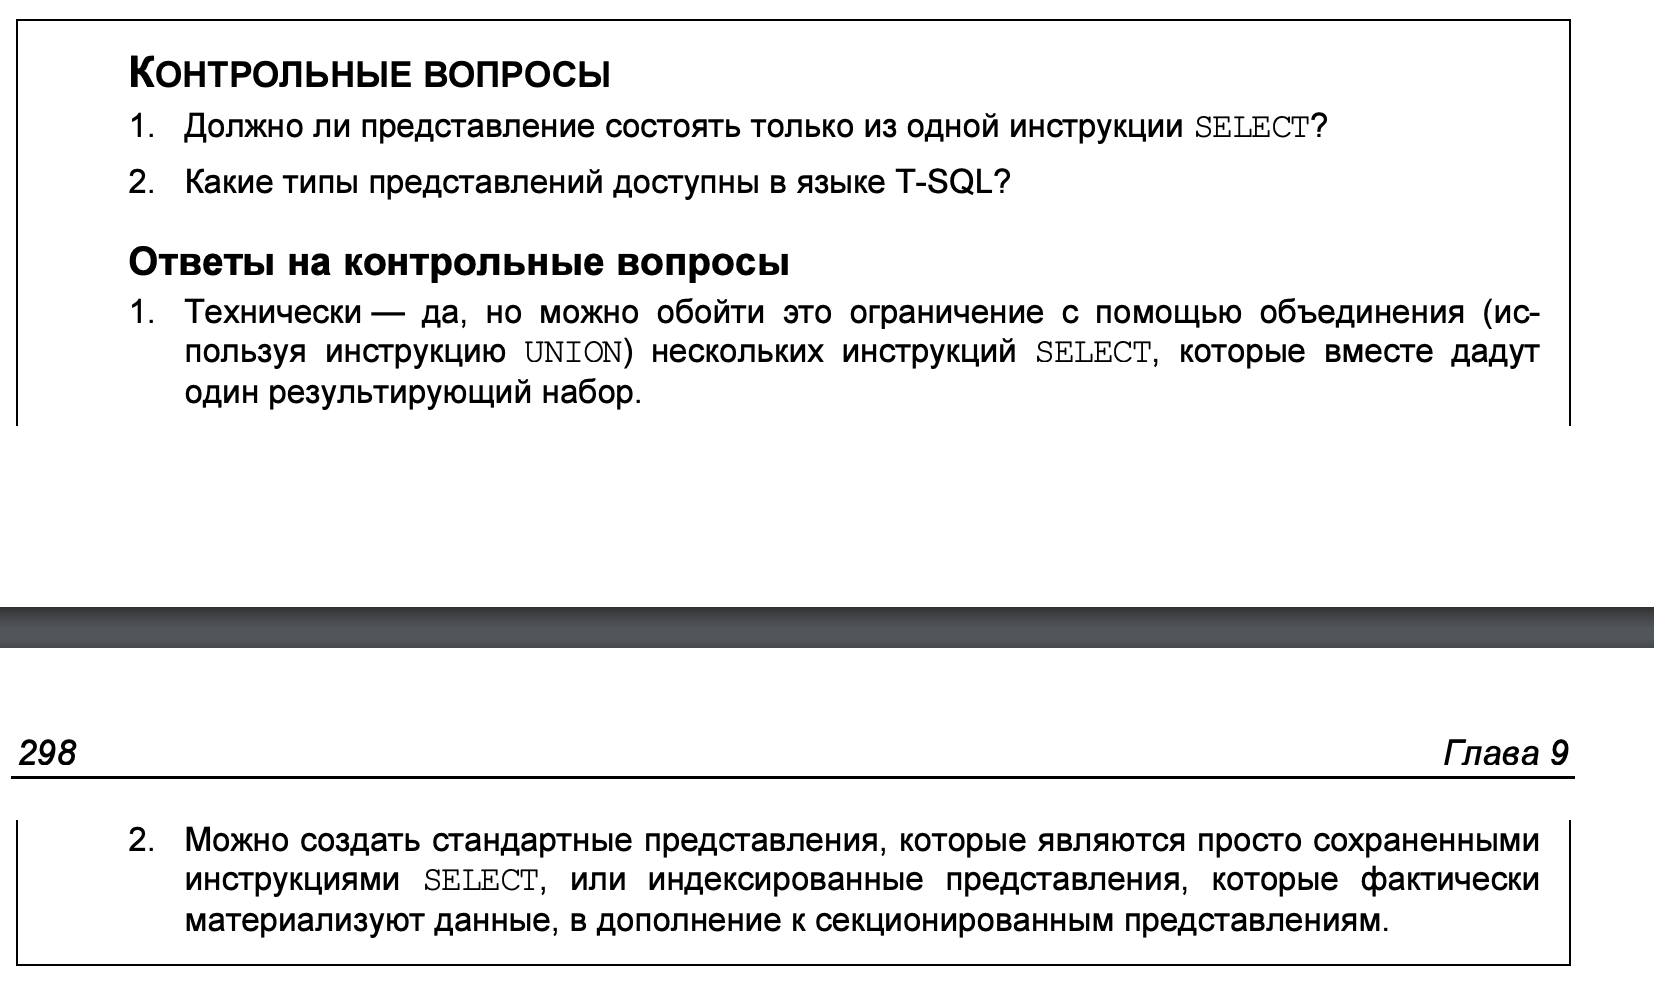
\includegraphics[width=0.9\textwidth]{img/control18.png}
	\end{center}
	\captionsetup{justification=centering}
\end{figure}


\subsection{Встроенные функции}

\begin{lstlisting}[label=lst:funcReturn, language=sql]
	CREATE FUNCTION Sales.fn_OrderTotalsByYear ()
	RETURNS TABLE
	AS
	RETURN
	( SELECT
	 YEAR(O.orderdate) AS orderyear,
	 SUM(OD.qty) AS qty
	 FROM Sales.Orders AS O
	 JOIN Sales.OrderDetails AS OD
	 ON OD.orderid = O.orderid
	 GROUP BY YEAR(orderdate)
	); 
\end{lstlisting}

Для создания встроенной табличной функции необходимо выполнить следующие
действия. 

\begin{itemize}
	\item Указать параметры. Параметры являются необязательными, но круглые скобки,
	в которые они должны быть заключены, обязательны. 
	\item Добавить предложение RETURNS TABLE, чтобы проинформировать SQL Server, что
	это табличная функция. 
	\item После блока AS ввести одну инструкцию RETURN. Она действует как встроенная
	функция для возвращения внедренной инструкции SELECT. 
	\item Внедрить инструкцию SELECT, которая будет определять, что функция должна
	возвратить в виде набора строк вызывающей стороне. 
\end{itemize}


\begin{lstlisting}[label=lst:funcReturn, language=sql]
	CREATE FUNCTION Sales.fn_OrderTotalsByYear (@orderyear int)
	RETURNS TABLE
	 AS
	 RETURN
	 ( SELECT orderyear, qty FROM Sales.OrderTotalsByYear
	 WHERE orderyear = @orderyear);
\end{lstlisting}

Вы можете запросить функцию с передачей года, который хотите видеть, следующим образом: 

\begin{lstlisting}[label=lst:funcReturn, language=sql]
	SELECT orderyear, qty FROM Sales.fn_OrderTotalsByYear(2007);
\end{lstlisting}

\subsection{Параметры встроенной функции}

Встроенные функции имеют два важных параметра, таких же, как и у представления. 

\begin{itemize}
	\item Можно создать функцию с использованием предложения WITH ENCRYPTION, затруднив для пользователя раскрытие текста SELECT для функции. 
	\item Можно добавить предложение WITH SCHEMABINDING, которое привязывает схемы
	таблицы базовых объектов, таких как таблицы или представления, к функции.
	Схемы объектов, на которые выполняется ссылка, не могут изменяться, пока
	функция не будет удалена или не будет удален параметр WITH SCHEMABINDING. 
\end{itemize}

\begin{figure}[h!]
	\begin{center}
		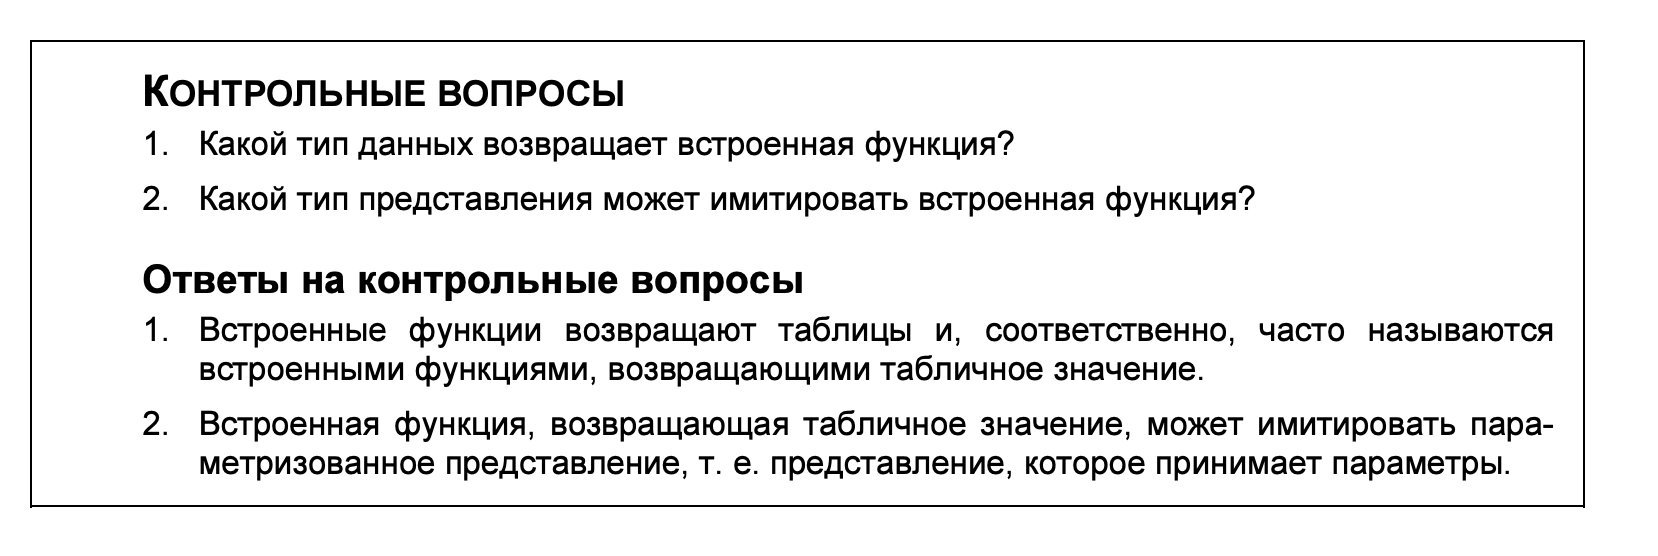
\includegraphics[width=0.9\textwidth]{img/control19.png}
	\end{center}
	\captionsetup{justification=centering}
\end{figure}


\subsection*{Резюме занятия}
\begin{itemize}
\item Представления — это сохраненные инструкции SELECT языка T-SQL, которые
могут обрабатываться, как если бы это были таблицы. 
\item Обычно представление состоит только из одной инструкции SELECT, но можно
обойти это правило, объединив инструкции SELECT со сходными результатами,
используя инструкции UNION или UNION ALL. 
\item Представления могут ссылаться на несколько таблиц и упростить сложные объединения для пользователей. 
\item По умолчанию представления не содержат никаких данных. Создание уникального кластеризованного индекса на представлении дает в результате индексированное представление, которое материализует данные. 
\item При выполнении выборки из представления SQL Server берет самую внешнюю
инструкцию SELECT и объединяет ее с инструкцией SELECT из определения представления. Затем SQL Server выполняет эту комбинированную инструкцию
SELECT. 
\item Можно модифицировать данные с помощью представления, но только для одной таблицы за один раз и лишь в столбцах определенных типов. 
\item Можно добавить к представлению предложение WITH CHECK OPTION для того,
чтобы предотвратить любые изменения через представление, которые могут
привести к получению в строках значений, не удовлетворяющих предложению
WHERE данного представления. 
\item Представления могут ссылаться на таблицы или представления в других базах
данных и на других серверах через связанные серверы.
\item Специальные представления, называемые секционированными представлениями, могут быть созданы при условии удовлетворения определенному набору
требований, и если SQL Server выполняет маршрутизацию соответствующих запросов и обновлений на нужную секцию представления. 
\item Встроенные функции можно использовать для имитации параметризованных
представлений. Представления языка T-SQL не могут принимать параметры. Но
встроенная функция, возвращающая табличное значение, может возвращать те
же данные, что и представление, а также принимать параметры, которые могут
фильтровать результаты. 
\end{itemize}


\subsection*{Закрепление материала}

\begin{figure}[h!]
	\begin{center}
		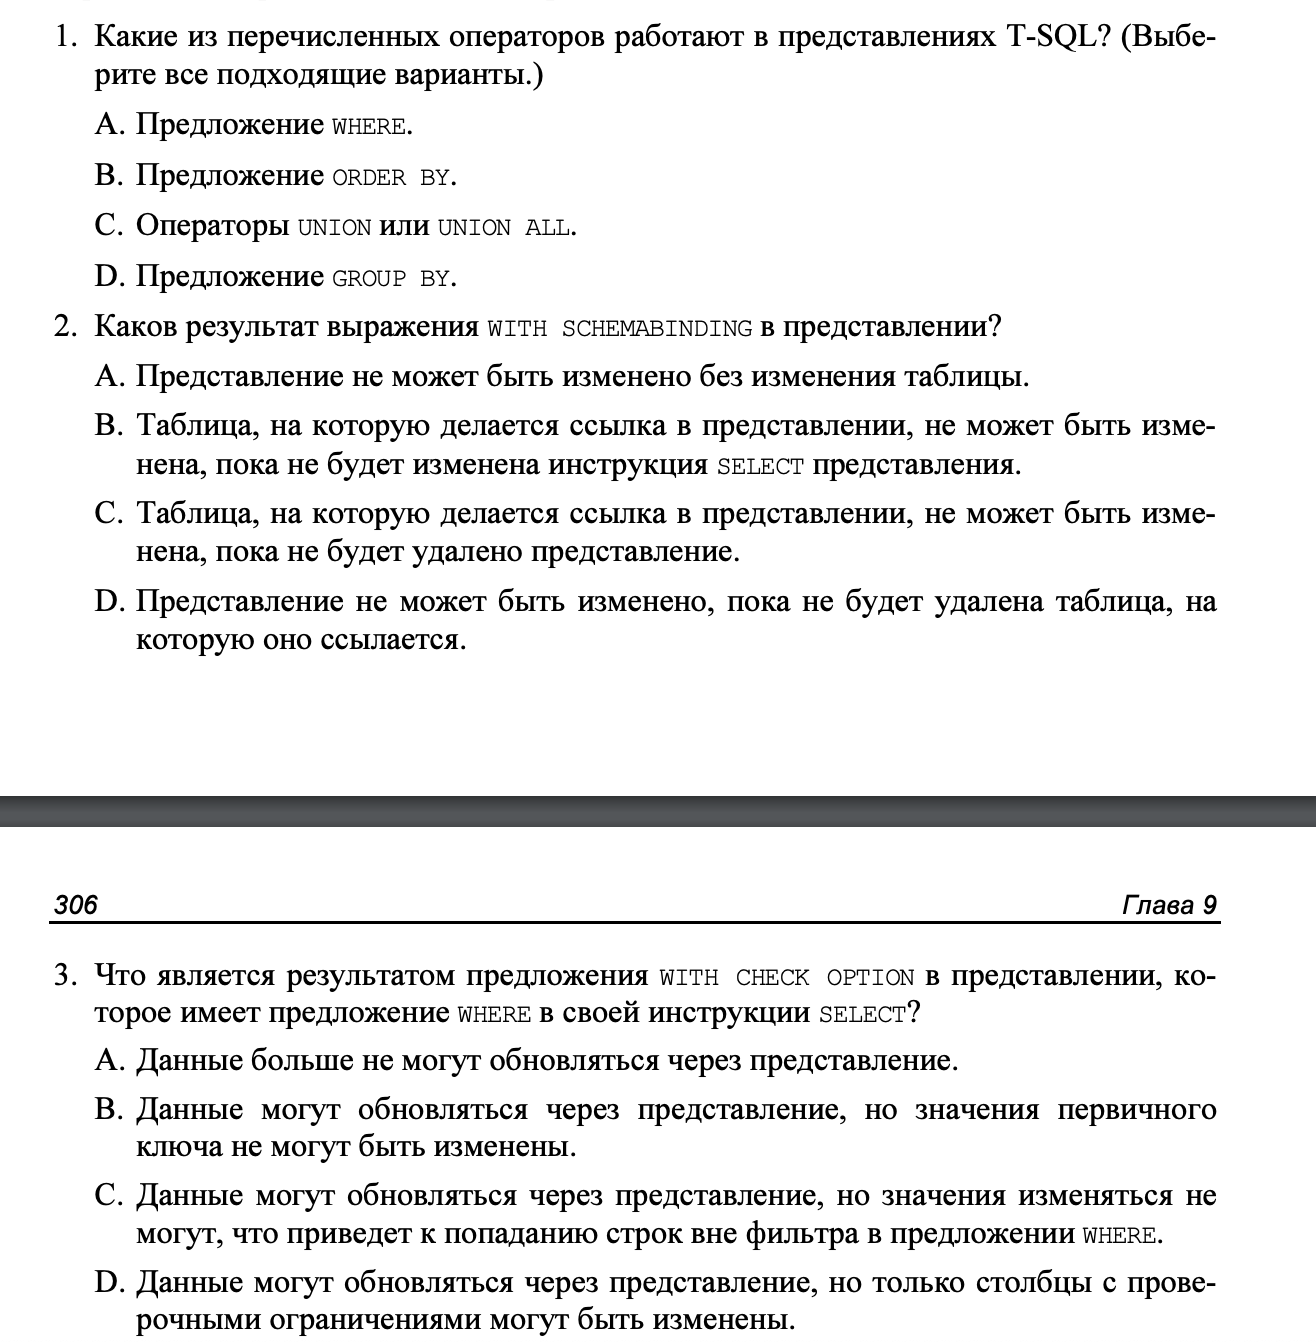
\includegraphics[width=0.9\textwidth]{img/zakrep17.png}
	\end{center}
	\captionsetup{justification=centering}
\end{figure}
\newpage

\subsection*{Ответы}

\begin{figure}[h!]
	\begin{center}
		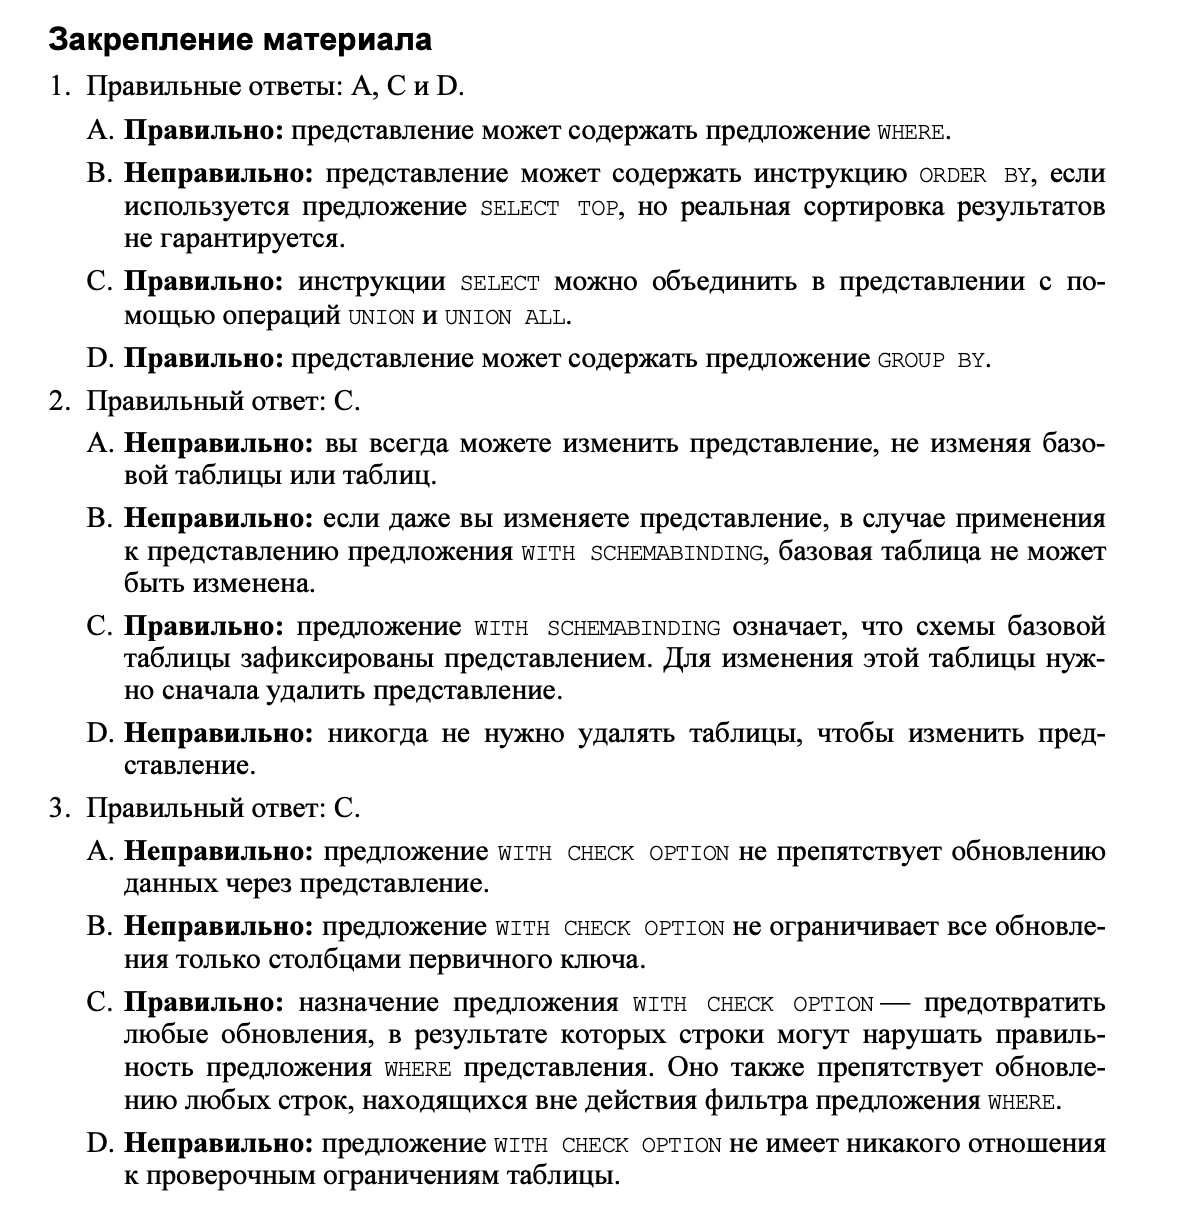
\includegraphics[width=0.9\textwidth]{img/ans19.png}
	\end{center}
	\captionsetup{justification=centering}
\end{figure}
\clearpage


\section{Использование синонимов}

Синонимы — это имена, сохраняемые в базе данных, которые могут
использоваться для замещения имен других объектов. Эти имена также действуют в пределах базы данных и добавляются к имени схемы. 


\subsection{Создание синонима}

\begin{lstlisting}[label=lst:funcReturn, language=sql]
	CREATE SYNONYM dbo.Categories FOR Production.Categories;
\end{lstlisting}	

Затем конечный пользователь может делать выборку из Categories без необходимости указывать схему. 

\begin{lstlisting}[label=lst:funcReturn, language=sql]
	SELECT categoryid, categoryname, description FROM Categories; 
\end{lstlisting}	

Синонимы могут применяться для следующих типов объектов: 

\begin{itemize}
	\item таблицы (включая временные таблицы); 
	\item представления; 
	\item пользовательские функции (скалярные, табличные, встроенные); 
	\item хранимые процедуры (T-SQL, расширенные хранимые процедуры и процедуры
	фильтра репликации); 
	\item сборки среды CLR (хранимые процедуры, табличные, скалярные и статистические функции). 
\end{itemize}

\begin{figure}[h!]
	\begin{center}
		
\includegraphics[width=0.9\textwidth]{img/advice19.png}
	\end{center}
	\captionsetup{justification=centering}
\end{figure}

\begin{figure}[h!]
	\begin{center}
		
\includegraphics[width=0.9\textwidth]{img/advice20.png}
	\end{center}
	\captionsetup{justification=centering}
\end{figure}

\subsection{Сравнение синонимов
с другими объектами баз данных}

Далее приведены преимущества синонимов перед представлениями. 
\begin{itemize}
	\item В отличие от представлений, синонимы могут замещать многие другие типы
	объектов базы данных, не только таблицы. 
	\item Также как и представления, синонимы могут предоставлять уровень абстракции,
	давая возможность создать логическое представление системы без необходимости показывать физические имена объектов базы данных конечному пользователю. Если базовый объект изменен, его синоним от этого не пострадает. 
	\item В отличие от представлений, синонимы не способны упростить сложную логику, как, например, представление может упростить сложные соединения. Синонимы в действительности — это просто имена. 
	\item Представление может ссылаться на множество таблиц, а синоним может ссылаться только на один объект. 
	\item Представление может ссылаться на другое представление, тогда как синоним
	не может ссылаться на другой синоним; создание цепочки синонимов недопустимо. 
\end{itemize}

Когда представление замещает таблицу, пользователь может видеть столбцы и типы данных представления. Но синоним не отображает метаданные базовой таблицы
или представления, которые он замещает. Это может быть как преимуществом, так
и недостатком, в зависимости от контекста.

\begin{itemize}
	\item Если вы не хотите предоставлять данные пользователю, это можно рассматривать как преимущество. В среде SSMS, когда пользователь открывает дерево,
	чтобы взглянуть на синоним, этот пользователь не увидит столбцов или типов
	данных, если синоним ссылается на таблицу или представление, а также пользователь не увидит никаких параметров, если синоним ссылается на процедуру
	или функцию.
	\item Если вы хотите предоставлять метаданные пользователю как часть его обучения,
	тогда синоним может быть недостатком. Например, пользователю могла бы понадобиться внешняя документация, чтобы выяснить, какие столбцы доступны. 
\end{itemize}

\begin{figure}[h!]
	\begin{center}
		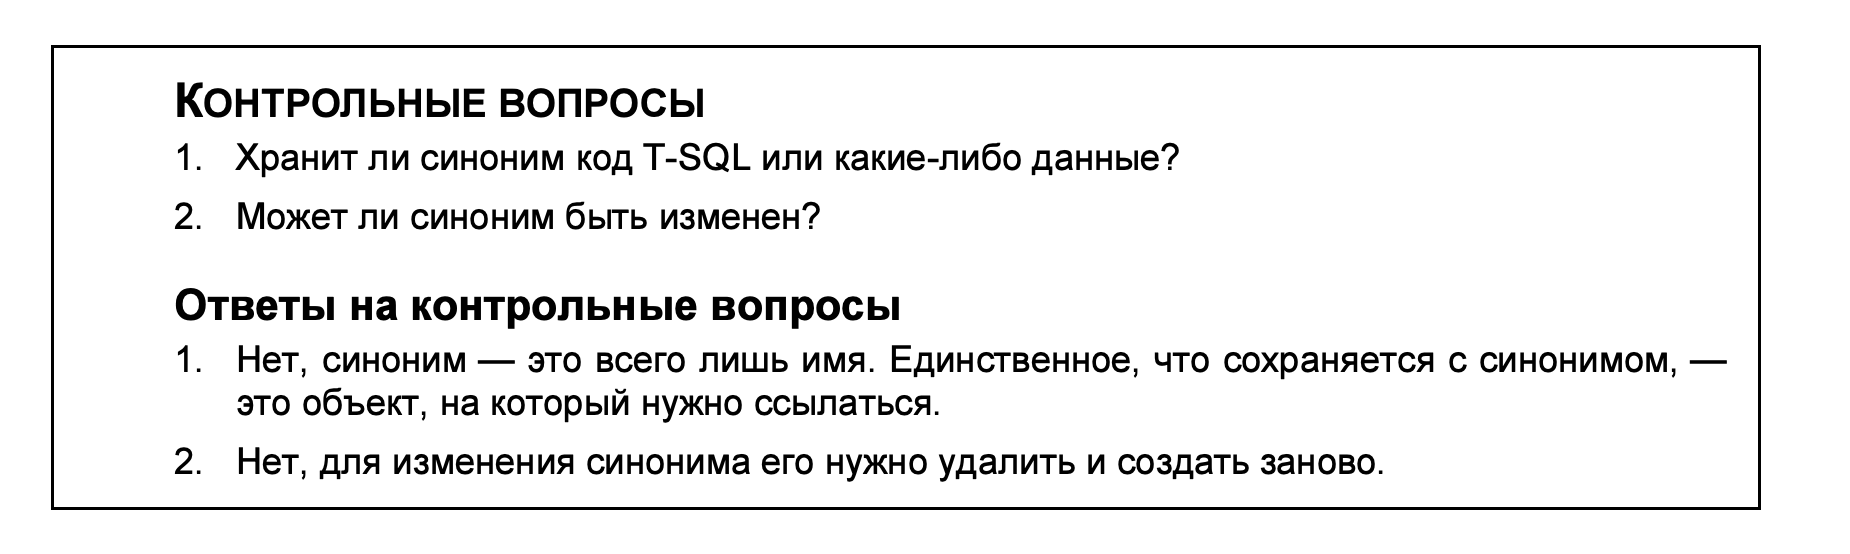
\includegraphics[width=0.9\textwidth]{img/control20.png}
	\end{center}
	\captionsetup{justification=centering}
\end{figure}


\subsection*{Резюме занятия}
\begin{itemize}
	\item Синоним — это имя, которое ссылается на другие объекты базы данных, такие
	как таблица, представление, функция или хранимая процедура. 
	\item Синоним не хранит никакого кода T-SQL и никаких данных. Он хранит только
	объект, на который выполняется ссылка.
	\item Синонимы находятся в области действия базы данных и поэтому существуют
	в том же пространстве имен, что и объекты, на которые они ссылаются. Следовательно, синониму нельзя дать то же имя, что и другому объекту базы данных. 
	\item Цепочки синонимов не разрешены; синоним не может ссылаться на другой
	синоним. 
	\item Синонимы не предоставляют никаких метаданных объектов, на которые они
	ссылаются. 
	\item Синонимы могут использоваться для предоставления уровня абстракции пользователю с помощью различных имен для объектов баз данных. 
	\item Можно модифицировать данные с помощью синонима, но нельзя изменить
	базовый объект. 
	\item Чтобы изменить синоним, его надо сначала удалить, а затем снова создать. 
\end{itemize}


\subsection*{Закрепление материала}

\begin{figure}[h!]
	\begin{center}
		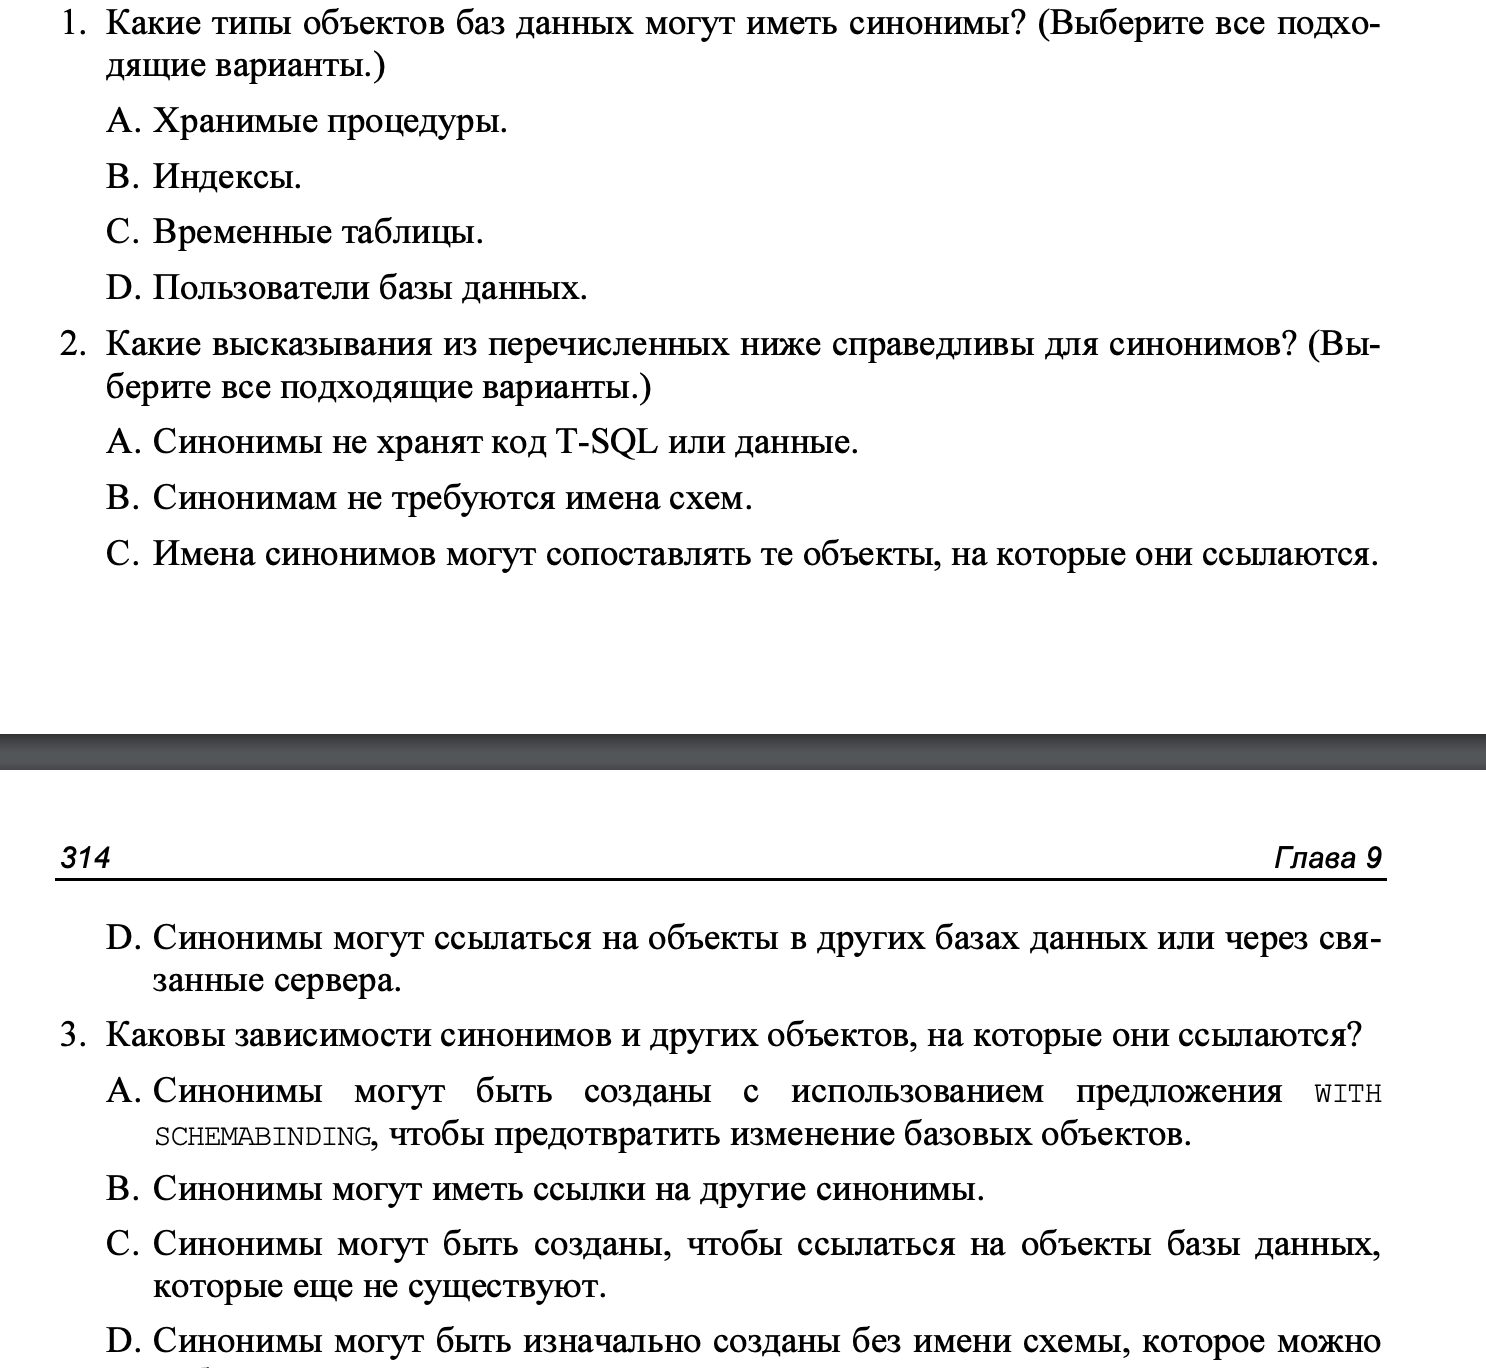
\includegraphics[width=0.9\textwidth]{img/zakrep18.png}
	\end{center}
	\captionsetup{justification=centering}
\end{figure}
\clearpage

\subsection*{Ответы}

\begin{figure}[h!]
	\begin{center}
		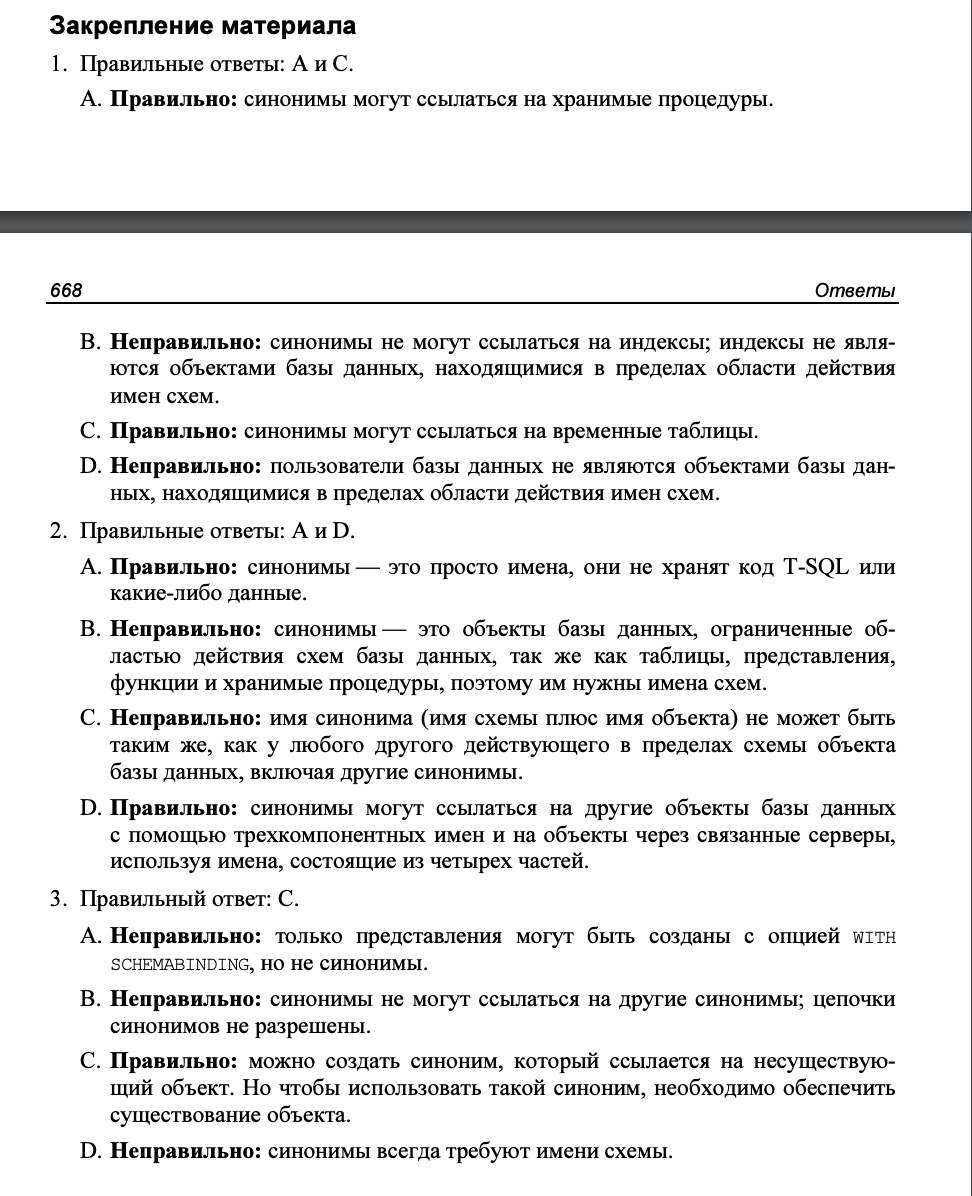
\includegraphics[width=0.9\textwidth]{img/ans20.png}
	\end{center}
	\captionsetup{justification=centering}
\end{figure}


\newpage
\subsection*{Упражнения}

\begin{figure}[h!]
	\begin{center}
		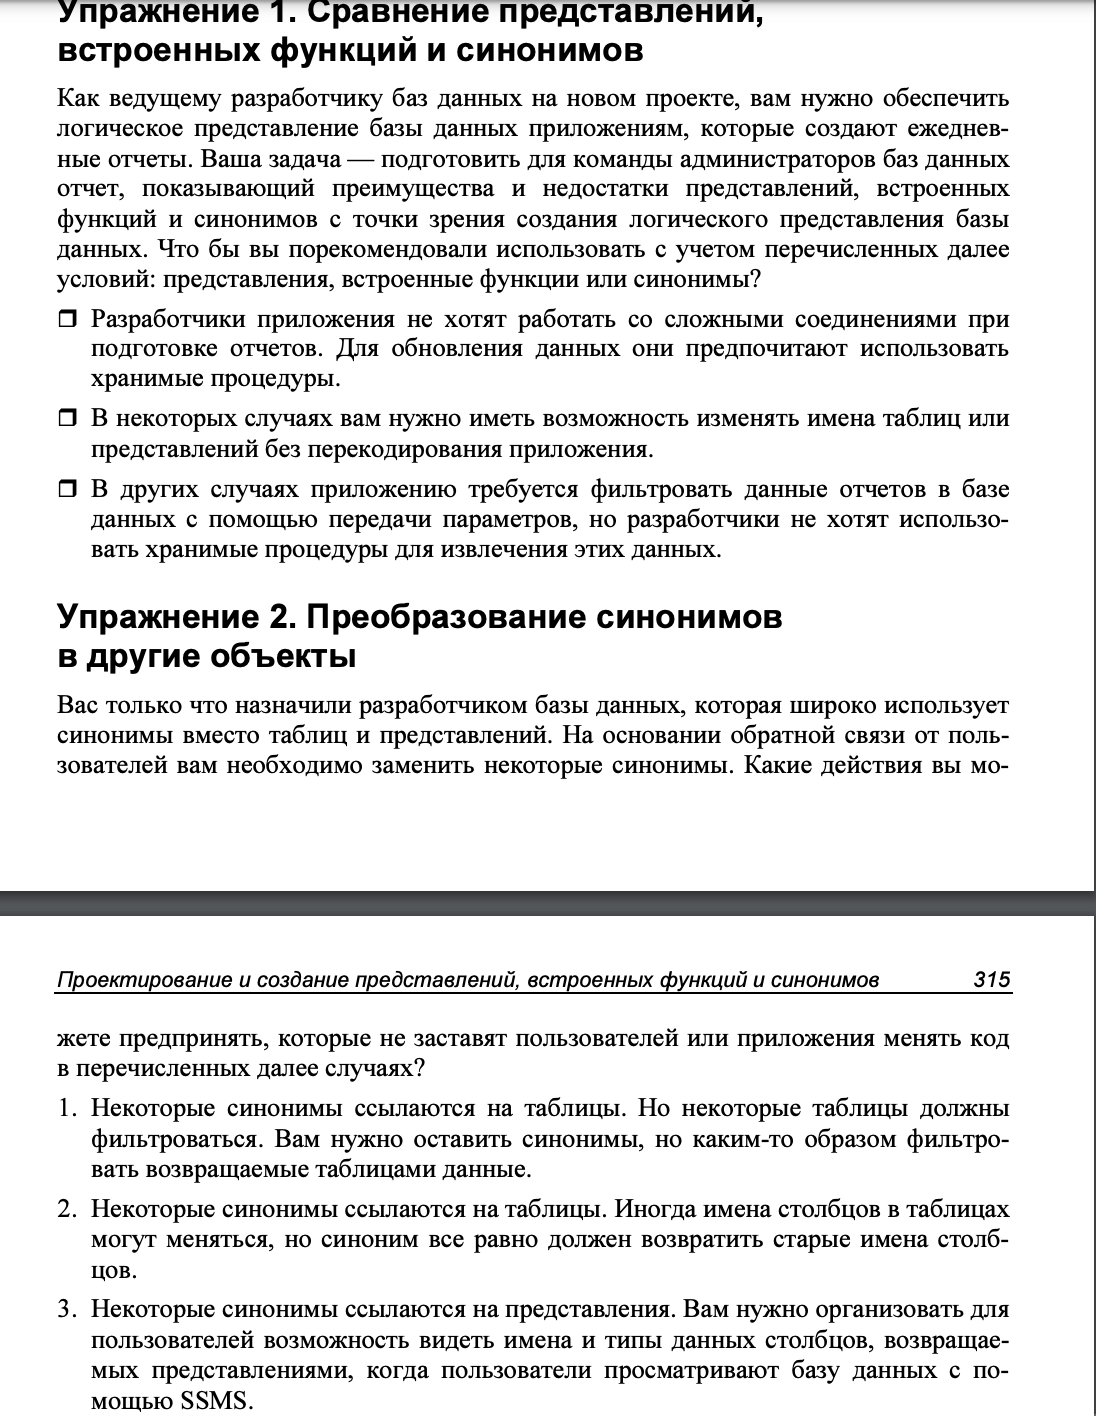
\includegraphics[width=0.9\textwidth]{img/ex15.png}
	\end{center}
	\captionsetup{justification=centering}
\end{figure}

\subsection*{Ответы}

\begin{figure}[h!]
	\begin{center}
		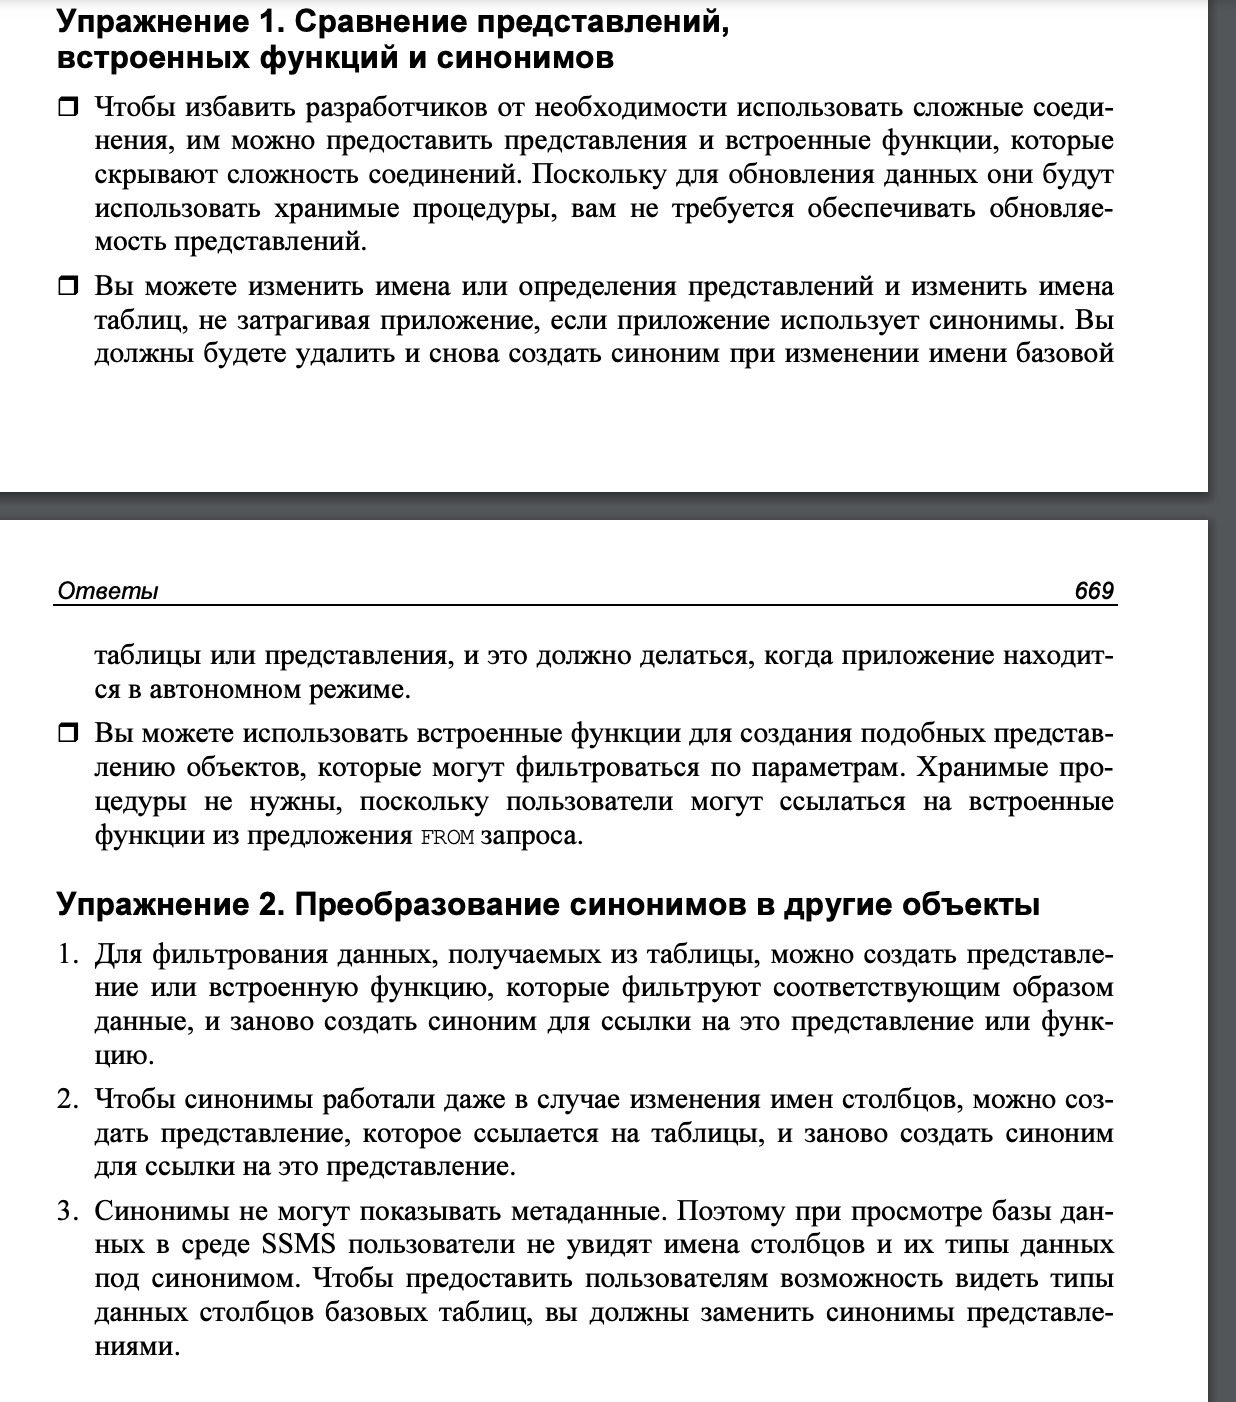
\includegraphics[width=0.9\textwidth]{img/eans15.png}
	\end{center}
	\captionsetup{justification=centering}
\end{figure}





